\chapter{La strategia finale: Top Vega}
\label{ch:strategia}

\section{Meccanismo economico}
\label{sec:strategia-meccanismo}

La strategia sopravvissuta al processo di eliminazione del
Capitolo~\ref{ch:percorso} è la più semplice tra quelle considerate: ogni
giorno seleziona e vende l'opzione con il vega più elevato nell'universo
filtrato. La motivazione economica è diretta. Il vega misura la sensibilità
del prezzo dell'opzione alla volatilità implicita; vendere l'opzione a vega
massimo significa massimizzare l'esposizione al premio per il rischio di
volatilità per unità di trade. Se il premio esiste, cioè se la volatilità
implicita eccede sistematicamente quella realizzata, allora concentrare
l'esposizione dove il vega è più alto è il modo più efficiente per
raccoglierlo. A differenza dei segnali esplorati nel
Capitolo~\ref{ch:percorso}, questa regola non contiene parametri da
stimare, non richiede il confronto tra densità e non pretende di prevedere
quando il premio sarà più ricco: si limita a raccoglierlo nel punto in cui
la sensibilità alla volatilità è massima.

Il profitto della strategia proviene da due fonti. La prima è la gamba
opzionaria: si incassa il premio e, se la volatilità realizzata resta
inferiore all'implicita prezzata, l'opzione decade a favore del venditore.
La seconda è la copertura delta: neutralizzando l'esposizione direzionale
con futures trimestrali e ribilanciando quotidianamente, la strategia
realizza un profitto dal ribilanciamento gamma quando il sottostante oscilla.
Come sarà quantificato nel Capitolo~\ref{ch:validazione}, su Bitcoin
l'81\% del profitto proviene dalla vendita di opzioni e il 19\% dalla
copertura: la strategia è dunque genuinamente una raccolta del premio di
volatilità, con la copertura che agisce da amplificatore su un sottostante
ad alta volatilità realizzata.

\section{Regole operative}
\label{sec:strategia-regole}

La Tabella~\ref{tab:configurazione} riassume la configurazione completa.

\begin{table}[H]
\centering
\caption{Configurazione completa della strategia Top Vega.}
\label{tab:configurazione}
\begin{tabular}{ll}
\toprule
\textbf{Componente} & \textbf{Regola} \\
\midrule
Selezione & opzione con $|\text{vega}|$ massimo, $|\Delta| \le 0{,}50$ \\
Posizioni & singola (max 1 aperta) \\
Entry & vendita al bid, esecuzione T+1 \\
Exit & riacquisto all'ask; profit target 50\% \emph{oppure} DTE $\le 5$ \\
Copertura & futures trimestrali Deribit, ribilanciamento giornaliero \\
Costi opzione & 0,03\% del sottostante per lato (cap Deribit) \\
Costi hedge & 0,10\% per lato (commissione, spread, slippage) \\
Stop loss & assente (controindicato, \S\ref{sec:percorso-stoploss}) \\
Filtri di regime & assenti (non predittivi, \S\ref{sec:percorso-regime}) \\
\bottomrule
\end{tabular}
\end{table}

Alcune scelte meritano una motivazione esplicita. Il filtro sul delta
($|\Delta| \le 0{,}50$) esclude le opzioni profondamente in-the-money, che
sul mercato Bitcoin sono illiquide e il cui prezzo nei dati è inaffidabile:
è la correzione che nel Capitolo~\ref{ch:percorso} ha smascherato
l'artefatto della strategia Premium/DTE. L'uscita a 5 giorni dalla scadenza
evita la zona in cui il gamma dell'opzione esplode e la copertura diventa
instabile e costosa. La scelta dei futures trimestrali per la copertura, in
luogo dei perpetui, elimina l'esposizione al tasso di funding, che nei
mercati rialzisti penalizza le posizioni corte. Il profit target al 50\% e
la soglia di uscita a 5 giorni sono parametri del backtest, non ottimizzati
sulla griglia di sensibilità: la robustezza della strategia alla loro
variazione è documentata nel Capitolo~\ref{ch:validazione}.

\section{Profilo dei trade selezionati}
\label{sec:strategia-profilo}

La regola Top Vega, pur non imponendo vincoli espliciti sulla scadenza o
sulla moneyness, seleziona in modo naturale un profilo di trade ben
definito, riassunto nella Tabella~\ref{tab:profilo-trade}. Poiché il vega di
un'opzione è massimo per strumenti vicini all'at-the-money e con scadenza
lontana, la strategia tende a vendere opzioni near-ATM (moneyness circa
1,04) con scadenza medio-lunga (DTE mediano all'ingresso di circa 66
giorni), mantenendole in media per 25 giorni. Questo profilo è coerente con
il meccanismo: sono proprio le opzioni ad alto vega quelle che offrono la
massima esposizione al premio di volatilità.

\begin{table}[H]
\centering
\caption{Profilo tipico dei trade selezionati dalla strategia Top Vega.}
\label{tab:profilo-trade}
\begin{tabular}{lc}
\toprule
\textbf{Metrica} & \textbf{Valore} \\
\midrule
DTE medio all'ingresso & $\sim$66 giorni \\
Moneyness & $\sim$1,04 (near-ATM) \\
IV media all'ingresso & $\sim$63\% \\
Holding period medio & $\sim$25 giorni \\
Vega per contratto & $\sim$49--98 \\
Meccanismo di profitto & raccolta del VRP (IV $>$ RV) \\
\bottomrule
\end{tabular}
\end{table}

\section{Risultati}
\label{sec:strategia-risultati}

La Tabella~\ref{tab:risultati-principali} riporta i risultati della
strategia nella configurazione di dimensionamento moderata (rischio 2\%,
buffer 1,5$\times$; il dimensionamento è trattato nel
Capitolo~\ref{ch:money-management}), su entrambi i periodi. Va sottolineato
fin d'ora che lo Sharpe ratio è invariante rispetto al dimensionamento,
poiché è un rapporto: le tre configurazioni di rischio scalano linearmente
rendimento e drawdown ma lasciano immutato lo Sharpe.

\begin{table}[H]
\centering
\caption{Risultati della strategia Top Vega, configurazione moderata
(rischio 2\%, buffer 1,5$\times$). Risultati post-audit.}
\label{tab:risultati-principali}
\begin{tabular}{lcc}
\toprule
\textbf{Metrica} & \textbf{In-sample} & \textbf{Out-of-sample} \\
\midrule
Trade & 35 & 10 \\
Sharpe ratio & 1,75 & 1,52 \\
Return & $+19{,}3\%$ & $+7{,}0\%$ \\
Max drawdown (MTM) & $-10{,}3\%$ & $-2{,}3\%$ \\
Win rate & 65,7\% & 70,0\% \\
t-test ($p$-value) & 0,007 & 0,091 \\
\bottomrule
\end{tabular}
\end{table}

\begin{figure}[H]
\centering
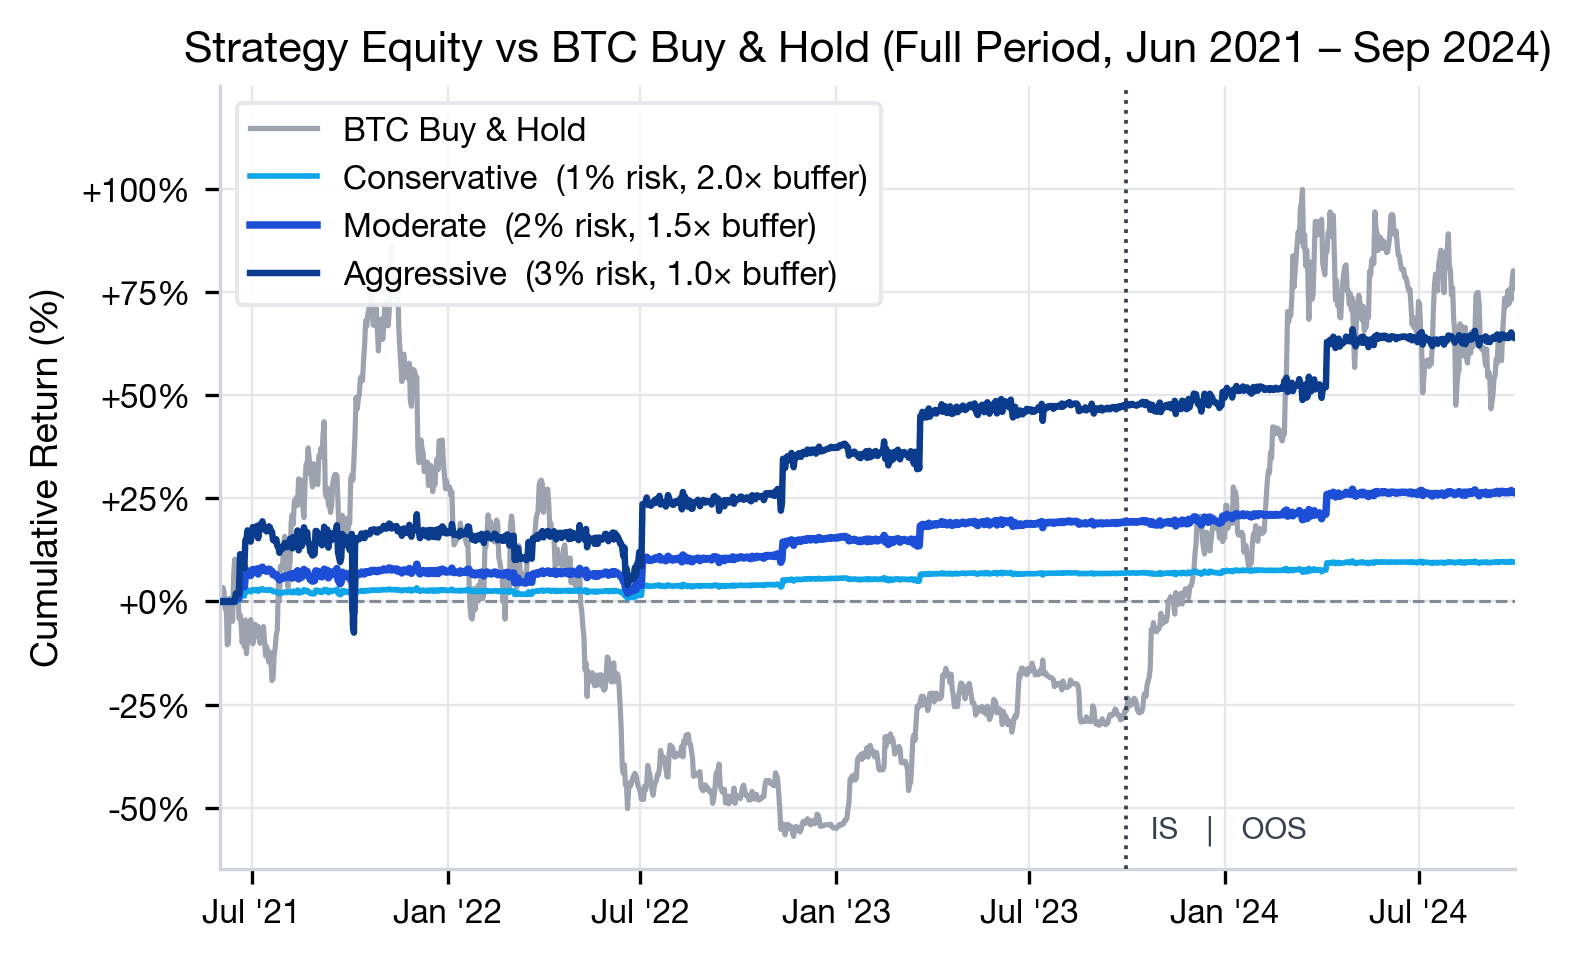
\includegraphics[width=\textwidth]{figures/fig2_equity.png}
\caption{Curva di equity mark-to-market della strategia Top Vega.}
\label{fig:equity}
\end{figure}

Il dato più solido è lo Sharpe in-sample di 1,75, ottenuto attraversando il
bear market del 2022 (Tabella~\ref{tab:contesto-mercato}). Come discusso nel
Capitolo~\ref{ch:dati}, l'in-sample è il periodo di prova più severo per una
strategia short volatility, proprio perché include l'episodio di stress cui
questa categoria di strategie è più esposta. Lo Sharpe out-of-sample, pari a
1,52, conferma la tenuta della strategia, ma va letto nel contesto di un
mercato rialzista con volatilità in compressione, favorevole alla vendita di
volatilità, e con soli 10 trade la sua stima è meno affidabile (il t-test
out-of-sample è significativo soltanto al 10\%). La validazione statistica
completa, comprensiva di intervalli di confidenza bootstrap e test di
robustezza, è sviluppata nel Capitolo~\ref{ch:validazione}.

Un'ultima osservazione riguarda la metrica di drawdown. I valori riportati
in tabella sono calcolati sulla curva mark-to-market, non sui soli trade
chiusi. Per una strategia che detiene posizioni in media per 25 giorni, il
drawdown mark-to-market è la misura onesta del rischio sopportato, perché
riflette le oscillazioni del valore della posizione lungo tutta la sua vita,
comprese le perdite non realizzate che, come mostrato
nella \S\ref{sec:percorso-stoploss}, i trade vincenti attraversano prima di
recuperare.
